\documentclass{report}
\usepackage[utf8]{inputenc}

\title{Statistical Inference for Entropy}
\author{Karina Marks}

\usepackage{amsmath, amsfonts, graphicx, listings, booktabs, amstext, subcaption}
\usepackage[format=plain,
            textfont=it]{caption}


\newtheorem{theorem}{Theorem}
\newtheorem{remark}{Condition}

\begin{document}
\chapter{Monte-Carlo Simulations}

In this chapter I will explore simulations of the bias of estimator (\ref{KLest}) in comparison to the size of the sample estimated from, with respect to different values of k; by exploring 1-dimensional distributions and then progressing onto 2-dimensional. Firstly, the distributions considered will be analysed to determine if they satisfy the conditions \ref{A1}, \ref{A2} and \ref{A3} stated for Theorems \ref{unbias} and \ref{efficient} to hold. Then, I will explore the estimator of entropy for simulations of samples from certain distributions, for different values of $k$.

The motivation for these simulations is to explore the consistency of this estimator for different values of $k$; the relationship between the size of the bias of the estimator $\hat{H}_{N, k}$, $Bias(\hat{H}_{N, k})$,  and the sample size, $N$. Throughout this analysis we will be considering the absolute value of this bias, since when taking its logarithm, we need a positive value. Using Theorem \ref{unbias}, we can write that the bias of the estimator approaches 0 as $N \to \infty$. This is because we can write $Bias(\hat{H}_{N, k} ) = \mathbb{E}(\hat{H}_{N, k}) - H$, which in equation (\ref{unbias_equation}) implies $Bias(\hat{H}_{N, k}) \to 0$ as $N \to \infty$. Thus, there must be a type of inverse relationship between the modulus of the bias of the estimator, $|Bias(\hat{H}_{N, k})|$, and $N$. We believe this relationship is of the form;
\begin{equation} \label{bias}
|Bias(\hat{H}_{N, k})| = \frac{c}{N^a}
\end{equation}
for $a, c > 0$ \cite{paper3, paper4}. By taking the logarithm of this, we can generate a linear relationship, which is easier to analyse, and is given by;
\begin{align} 
log|Bias(\hat{H}_{N, k})| &\approx log(c) - a [log(N)] + \epsilon \nonumber \\
&\approx \zeta - a [log(N)] \label{logbias}
\end{align}
where $\epsilon > 0$ is some small error term. I will investigate the consistency of this estimator for a sample from a specified distribution, dependent on the value of $k$, this mean finding the optimum value of $k$ for which $|Bias(\hat{H}_{N, k})| \to 0$ for $N \to \infty$. For the relationship in equation (\ref{bias}), this will happen for larger values of $a$ and relatively small $c$, as $N \to \infty$. As previously mentioned, there is evidence supporting that the bias becomes either of order $(\frac{1}{N})^a$ (equation (\ref{fixedkbias})) or $(\frac{k}{N})^a$ (equation (\ref{dependentkbias})). This leads to also examining the dependence of $c$ / $\zeta$ on the value of $k$. 

As I wish to consider the difference in accuracy of the estimator when using different values of k, let us denote the approximate values for $a$ and $c$ dependent on $k$ as $a_{k}$ and $c_{k}$.

I will conduct a range of analysis, for each distribution, to consider how this estimator acts in reality, the process of analysis will be as follows;
\begin{enumerate}
\item Create a summary table of the mean absolute value of the bias of the estimator for $N=100, 25000$ and $50000$ for all values of $k$ that satisfy Condition \ref{A3}. I could also consider the variance of the bias at the values of $N$ stated above, for all applicable values of $k$. However, we will find that the $Var|Bias(\hat{H}_{50000, k})| \to 0$ for $k \to 10$, by the definition of the estimator using the nearest neighbour method. Taking a larger $k$ in the nearest neighbour method will produce less varied results, this is because more smoothing takes place for a larger $k$, eventually - if $k$ is made large enough - the output will be constant and the variance negligible regardless of the inputted values. Thus, considering the variance of the bias of the estimator in comparison to $k$ is not necessarily informative. 

\item Graphical representations of the linear relationship shown in equation \ref{logbias}, of $log(N)$ against $log|Bias(\hat{H}_{N, k})|$ for sample sizes $N=100, 200, 300, ..., 50000$ (which are taken $500$ times and averaged), for each value of $k$.

\item Tabulate the results from the regression analysis; I will first discuss the coefficient of determination ($R^2$), this is a measure
of how well the regression model describes the observed data \cite{regression1}. Next I will consider the standard error/deviation of the model ($\sigma^2$), this is a measure of accuracy of predictions. Lastly, I will go onto consider the values of $a_{k}$ and $c_{k}$ from relationship shown in equation \ref{bias}, for each $k$, which is the regression line that minimizes the sum of squared deviations ($\sigma^2$) of prediction.

\item Graphically compare the values of $a_{k}$ and $c_{k}$ for each $k$.

\end{enumerate}



\section{1-dimensional Gaussian/Normal Distribution} \label{Normal_d=1}

I will begin by exploring entropy of samples from the normal distribution $N(0, \sigma^2)$, where without loss of generality we can use the mean $\mu = 0$ and change the variance $\sigma^2$ as needed. The normal distribution has an exact formula to work out the entropy, given the variance $\sigma^2$. Using equation (\ref{ShaEnt}) and the density function for the normal distribution $f(x) = \frac{1}{\sqrt{(2\pi)} \sigma}\exp{ \left( \frac{-x^2}{2\sigma^2} \right)}$ for $x \in \mathbb{R}$, given $\mu = 0$. We can write the exact entropy for the normal distribution, using equation (\ref{ShaEnt});
\begin{align}
H &= - \int_{x \in \mathbb{R}^d} f(x) log(f(x)) dx \nonumber \\
&= - \int_{\mathbb{R}} \frac{1}{\sqrt{(2\pi)} \sigma}\exp{ \left( \frac{-x^2}{2\sigma^2} \right)} log \left[\frac{1}{\sqrt{(2\pi)} \sigma}\exp{ \left( \frac{-x^2}{2\sigma^2} \right)} \right] dx \nonumber \\
&=  \int_{\mathbb{R}} \frac{1}{\sqrt{(2\pi)} \sigma}\exp{ \left( \frac{-x^2}{2\sigma^2} \right)} \left( log(\sqrt{(2\pi)}\sigma) +  \frac{x^2}{2\sigma^2} \right) \nonumber \\
&= \frac{log(\sqrt{(2\pi)}\sigma)}{\sqrt{(2\pi)} \sigma} \int_{\mathbb{R}} \exp{ \left( \frac{-x^2}{2\sigma^2} \right)} dx +  \frac{1}{2\sqrt{(2\pi)} \sigma} \int_{\mathbb{R}} \frac{x^2}{2\sigma^2}  \exp{ \left( \frac{-x^2}{\sigma^2} \right)} dx \nonumber \\
&=  log(\sqrt{(2\pi)}\sigma) + \frac{1}{2} \nonumber 
\end{align}
Thus the exact entropy for the normal distribution is given by 
\begin{equation}\label{NormalEnt}
H =  log(\sqrt{(2\pi e)}\sigma) 
\end{equation}
I will first explore samples from 1-dimensional standard normal distribution with mean $\mu = 0$ and variance $\sigma^2 = 1$, $N(0, 1)$, to consider the behavior of the Kozachenko-Leonenko estimator. The exact entropy of this distribution is given by equation (\ref{NormalEnt}), with $\sigma^2=1$;
\begin{equation} \label{normal_exact}
H = log(\sqrt{(2\pi e)}) \approx 1.418939
\end{equation}

Since, I am first considering the 1-dimensional normal distribution, the estimator takes the form in equation (\ref{KLest_d=1}), which is given by;
\begin{equation}
\hat{H}_{N, k} =  \frac{1}{N} \sum_{i=1}^{N} log \left[ \frac{2\rho_{(k),i}(N-1)}{e^{\Psi(k)}} \right]\nonumber
\end{equation}







\subsection{Estimator Conditions} 

The density of the normal distribution satisfies Conditions \ref{A1}, \ref{A2} and \ref{A3}, due to the below analysis. Firstly, to satisfy Condition \ref{A1}, for density function $f(x) = \frac{1}{\sqrt{(2\pi)}} \exp{ \left( \frac{-x^2}{2} \right)}$ for $x \in \mathbb{R}$, given $\mu = 0$ and $\sigma^2 = 1$, it must be such that;
\begin{itemize}
\item $f$ is bounded - obvious, since for any probability distribution we always have $f(x) \geq 0$, additionally for the normal distribution we have that $f(x) = \frac{1}{\sqrt{(2\pi)}} \exp{ \left( \frac{-x^2}{2} \right)} < 0.4$, $\forall x \in \mathbb{R}$. Hence, $f$ is bounded above and below; so bounded.

\item $f$ is m-times differentiable - using Hermite polynomials, defined as;
\begin{equation}
H_{m}(x) = (-1)^m e^{\frac{x^2}{2}} \frac{d^m}{dx^m} \left(e^{\frac{-x^2}{2}} \right) \nonumber
\end{equation}
multiplying this by the coefficient in the distribution of $f(x)$, $\frac{1}{\sqrt(2 \pi}$, we then get;
\begin{align*}
 \frac{d^m}{dx^m} f(x) &= \frac{H_{m}(x)}{(-1)^m} \frac{1}{\sqrt{2 \pi}} e^{\frac{-x^2}{2}} \\ 
&= \frac{H_{m}(x)}{(-1)^m} f(x) 
\end{align*}
where $\frac{H_{m}(x)}{(-1)^m}$ is a polynomial; thus $f$ is m-times differentiable.

\item $\exists r_{*} > 0$ and a Borel measurable function $g_{*}$, with $\|y-x\| \leq r_{*}$ so that $\|f^{(t)}(x)\| \leq g_{*}(x) f(x)$ and $\|f^{(m)}(x) - f^{(m)}(x)\| \leq g_{*}(x) f(x)\|y - x\|^{\eta}$, for some $g_{*}$ such that $\sup_{\{x : f(x) < \delta\}} g_{*}(x) = O(\delta^{-\epsilon})$ as $\delta \searrow 0$ for some $\epsilon >0$. 

Since we are considering a 1-dimensional distribution, we can write the norms $\| \cdotp \|$ as  $| \cdotp |$. Moreover, considering that for Theorems \ref{unbias} and \ref{efficient}, we have the value of $\beta \geq 2$; thus choosing $\beta = 2$, and since $m = \lfloor \beta \rfloor =  \lfloor 2 \rfloor = 2 = \beta$ and $\eta = \beta -m$, we have that $\eta =0$. Thus we need  $|f^{(t)}(x)| \leq g_{*}(x) f(x)$, which is obvious by above, in view of writing $|\frac{d^t}{dx^t} f(x)| = g_{*}(x) f(x)$, where we choose $ g_{*}(x) = |\frac{H_{t}(x)}{(-1)^t}| = |H_{t}(x)|$, for $t=1,2,...,m$, and $|f(x)| = f(x)$, since $f(x) >0$. Also, $g_{*}$ is a polynomial and is hence Borel measurable over $\mathbb{R}$, and for any polynomial we obviously have $\sup_{\{x : f(x) < \delta\}} g_{*}(x) = O(\delta^{-\epsilon})$ as $\delta \searrow 0$ for some $\epsilon >0$. Additionally, we need $|f^{(m)}(x) - f^{(m)}(x)| \leq g_{*}(x) f(x)|y - x|^{0} = g_{*}(x) f(x)$. We currently have;
\begin{align*}
|f^{(m)}(x) - f^{(m)}(x)| &= \left| \frac{H_{m}(x)}{(-1)^m} f(x) - \frac{H_{m}(y)}{(-1)^m} f(y) \right| \\
&\leq \left| \frac{H_{m}(x)}{(-1)^m} f(x) \right| + \left| \frac{H_{m}(y)}{(-1)^m} f(y) \right| \\
&= g_{*}(x)f(x) + g_{*}(y)f(y) \\
&\leq g_{*}(x)f(x)
\end{align*}
since we know that $f(x) >0$ for all $x \in \mathbb{R}$, and $g_{*}(x) = |H_{m}(x)| >0$, which is similar to the $g_{*}$ before; thus satisfies the conditions for it.
\end{itemize}

Next, to satisfy Condition \ref{A2}, for the density function $f$ of the normal distribution, must fulfill that;
\begin{itemize}
\item The $\alpha$-moment of $f$ must be finite, so $\int_{\mathbb{R}^{d}} \| x \|^{\alpha} f(x) dx < \infty$ - this is always true for the normal distribution, all of its moments are finite, since they are defined with respect to $\sigma^n$, for some $n$, and $\sigma < \infty$.

\end{itemize}

Lastly, to satisfy Condition \ref{A3}, we must find the values of $k$ for which the estimator provides a uniform convergence for Theorems \ref{unbias} and \ref{efficient}. To do this we must have, for some $\alpha > d = 1$, let $k_{0}^{*}$ and $k_{1}^{*}$ denote two deterministic sequences of positive integers with $k_{0}^{*} \leq k_{1}^{*}$. Taking $\alpha := 2$, we must have;

\begin{itemize}
\item $k_{1}^{*} = O(N^{\tau})$, where $\tau < \min \left\{ \frac{2 \alpha}{5 \alpha + 3d} , \frac{\alpha - d}{2 \alpha} , \frac{4}{4 + 3d} \right\} = \min \left\{ \frac{4}{13}, \frac{1}{4}, \frac{4}{7} \right\} = \frac{1}{4}$, so we can choose $\tau := \frac{2}{9} < \frac{1}{4}$ so that we have $k_{1}^{*} = O(N^{\frac{2}{9}})$

\item $\frac{k_{0}^{*}}{\log^{5}{N}} \to \infty$ - for this to be true we need to choose $k_{0}^{*} := N^A$ for some $A>0$. Considering that $k_{0}^{*} \leq k_{1}^{*}$ and $ k_{1}^{*} = O(N^{\frac{2}{9}})$, thus $A \in (0, \frac{2}{9})$. So we can choose $A := \frac{1}{\eta}$ for some large $\eta$, which gives that $k_{0}^{*} = O(N^{\frac{1}{\eta}}) \approx 1$.
\end{itemize}

Thus, on account of the values of $N$ being considered in the simulations; $N=100, 200, ..., 50000$, we have that for the smallest $N=100$, the values of $k$ for which Theorem \ref{unbias} and \ref{efficient} both hold, are $k \in \{k_{0}^{*}, ..., k_{1}^{*} \} = \{1, ... , 100^{\frac{2}{9}}\} = \{1, ..., 2.782\} \approx \{1, 2\}$. Also, for the middle value $N=25,000$, we have the values of $k$ to be in $\{k_{0}^{*}, ..., k_{1}^{*} \}$, where $ k_{1}^{*} \approx 25000^{\frac{2}{9}} = 9.491 \approx 9$, thus $k \in \{ 1, ..., 9\}$. Moreover, for the largest $N=50,000$, we must consider $k \in \{1, ..., k_{1}^{*} \} = \{1, ... , 50000^{\frac{2}{9}}\} = \{1, ..., 11.072\} \approx \{1, 2, ..., 11\}$.

Overall, due to Conditions \ref{A1}, \ref{A2} and \ref{A3} being met, we can say that for the normal distribution, Theorems \ref{unbias} and \ref{efficient} hold; henceforth, we can say that the Kozachenko-Leonenko estimator, of a sample from the 1-dimensional normal distribution is an asymptotically unbiased and consistent estimator for entropy, for some values of $k \in \{1, 2, ..., 11\}$, depending on the sample size $N$. 






\subsection{Simulation Results}

I will now conduct some simulations to consider this for each value of $k$ separately, each time considering $500$ samples of size $N$ from this distribution, finding the estimator in each case and take the average of these estimators to find our entropy estimator. I will then consider the relationship show in equation (\ref{logbias}) for each sample and work out the average for the values of a and c, for each $k \in \{1, 2, ..., 11\}$. 

For $N=100$, $N=25,000$ and $N=50,000$, using the results from \ref{TODO-appendix data}, we can create a table to compare the mean values of the bias of the estimator for the different values of $k$ considered. 

\begin{table}
\caption{1-dimensional normal distribution, comparison of $k$} \label{normal_kcompare_table}
\begin{center}
\begin{tabular}{| l | c c c |} 
\toprule
$k$ &  $|Bias(\hat{H}_{100, k})|$ & $|Bias(\hat{H}_{25000, k})|$  &  $|Bias(\hat{H}_{50000, k})|$ \\
\midrule[1pt]
1     & 0.0031912    & 0.0006312    & 0.0004428   \\
2     & 0.0195347    & 0.0000092    & 0.0003632   \\
3     & 0.0167902    & 0.0000056    & 0.0002278   \\
4     & 0.0264708    & 0.0001657    & 0.0001196   \\
5     & 0.0238265    & 0.0002138    & 0.0000003   \\
6     & 0.0311576    & 0.0001546    & 0.0001471   \\
7     & 0.0356302    & 0.0000217    & 0.0003024   \\
8     & 0.0396299    & 0.0000984    & 0.0001021   \\
9     & 0.0460706    & 0.0003620    & 0.0002070   \\
10    & 0.0458648    & 0.0002752    & 0.0002611   \\
11    & 0.0387339    & 0.0003332    & 0.0002458   \\
\hline
\end{tabular}
\\[10pt]
\caption*{This table is comparing the values of $|Bias(\hat{H}_{N, k})|$ for the values of $k$ with $N=100$, $N=25,000$ and $N=50,000$, when the estimator is taken over $500$ samples}
\end{center}
\end{table}

The results shown in table \ref{normal_kcompare_table} show that for a larger $N$, the modulus of the bias of the estimator is smaller, this is true for all values of $k$ except when $k=2, 3, 7, 8$, for which the bias is smaller when $N=25,000$ in comparison to the larger value of $N$. There are a number of reasons why this could be; however, it is first important to notice that when finding the values of $k$ that satisfy condition\ref{A3}, we found that for $N=100$, we must have $k \in \{1, 2\}$, for $N=25,000$ we have $k \in \{1, 2, ..., 9 \}$ and for $N=50,000$ we have $k \in \{1, 2, ..., 11\}$.

For the smallest values of $N=100$, we expect the best value of $k$ to be either $1$ or $2$; and the table agrees with this showing that the smallest bias occurs at $k=1$ for a small sample size. 

When $N=25,000$ we have that for $k \in \{2,..., 8\}$ that the bias is very small, especially for the values of $k=3, 4, 7, 8$ with the smallest bias appearing when $k=3$; which fits with the previous analysis that the best value of $k$ will lie within $1$ and $9$.

Now considering the largest sample size $N=50,000$, the bias when $k=5$ sticks out since it is $\approx 10^{-3}$ smaller than the other bias values in the table. However, for all other values of $k$ the bias is still extremely small in comparison to the bias for $N=100$ and even in comparison to $N=25,000$ in some places. This extreme difference could be an outlier in my data; thus in table \ref{normal_k5_table} I have shown the values for the modulus of the bias, when $k=5$, for different, also large values of $N$. This table does indeed show that $|Bias(\hat{H}_{50000, 5})| \approx 0.0000003$ is an anomaly in the data, and that $k=5$ is not necessarily the best value of $k$ for $N=50,000$. Thus, we cannot yet draw any major conclusions about the best value of $k$ for the estimator of a sample this size.

\begin{table}
\caption{1-dimensional normal distribution, $k=5$ for large N} \label{normal_k5_table}
\begin{center}
\begin{tabular}{| l | c |} 
\toprule
$N$ &  $|Bias(\hat{H}_{N, 5})|$ \\
\midrule[1pt]
49100    & 0.0000639   \\
49200    & 0.0001463   \\
49300    & 0.0001700   \\
49400    & 0.0001037   \\
49500    & 0.0000711   \\
49600    & 0.0003221   \\
49700    & 0.0001047   \\
49800    & 0.0000644   \\
49900    & 0.0001240   \\
50000    & 0.0000003   \\
\hline
\end{tabular}
\\[10pt]
\caption*{This table is comparing the values of $Var|Bias(\hat{H}_{N, 5})|$ for the large values of $N$.}
\end{center}
\end{table}

I now wish to consider the equation \ref{logbias} and plot the simulated data, to fit a regression line for each value of $k$ separately, these are shown in Figures \ref{normal_graphs16} and \ref{normal_graphs711}. All of these graphs agree with the relationship previously stated between the sample size and the bias of the estimator; they all show that the logarithm of this equations gives a negative linear relationship - with relatively small error bars.

\begin{figure}
\makebox[\linewidth][c]{%
\begin{subfigure}[b]{.8\textwidth}
\centering
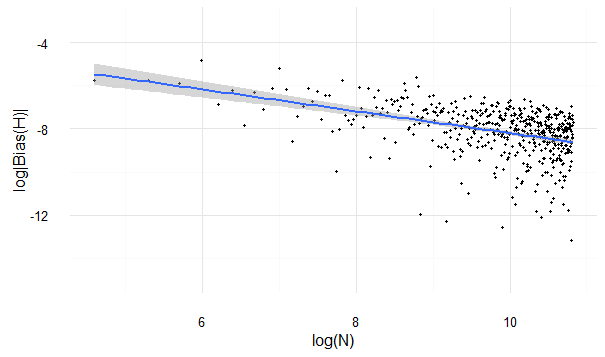
\includegraphics[width=\textwidth]{./Graphs/Best/Normal_k=1.png}\label{normal_k=1}
\caption{k=1}
\end{subfigure}%
\begin{subfigure}[b]{.8\textwidth}
\centering
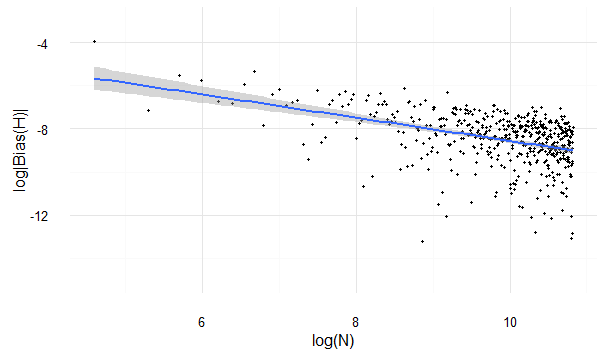
\includegraphics[width=\textwidth]{./Graphs/Best/Normal_k=2.png}\label{normal_k=2}
\caption{k=2}
\end{subfigure}%
}\    \makebox[\linewidth][c]{%
\begin{subfigure}[b]{.8\textwidth}
\centering
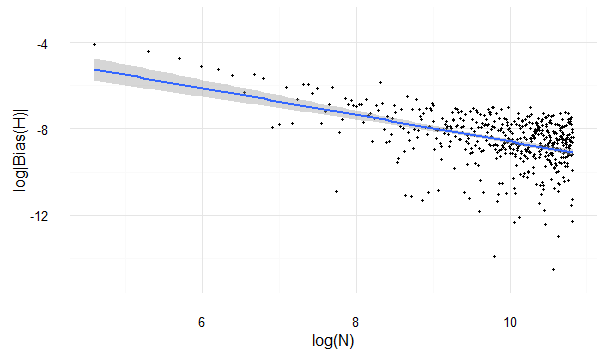
\includegraphics[width=\textwidth]{./Graphs/Best/Normal_k=3.png}\label{normal_k=3}
\caption{k=3}
\end{subfigure}%
\begin{subfigure}[b]{.8\textwidth}
\centering
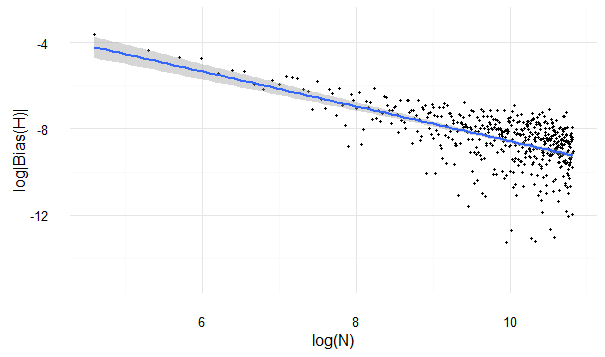
\includegraphics[width=\textwidth]{./Graphs/Best/Normal_k=4.png}\label{normal_k=4}
\caption{k=4}
\end{subfigure}%
}\    \makebox[\linewidth][c]{%
\begin{subfigure}[b]{.8\textwidth}
\centering
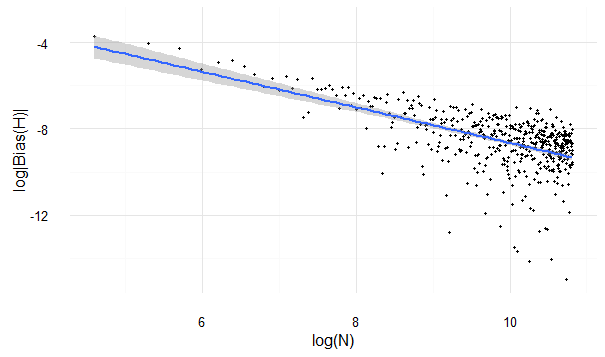
\includegraphics[width=\textwidth]{./Graphs/Best/Normal_k=5.png}\label{normal_k=5}
\caption{k=5}
\end{subfigure}%
\begin{subfigure}[b]{.8\textwidth}
\centering
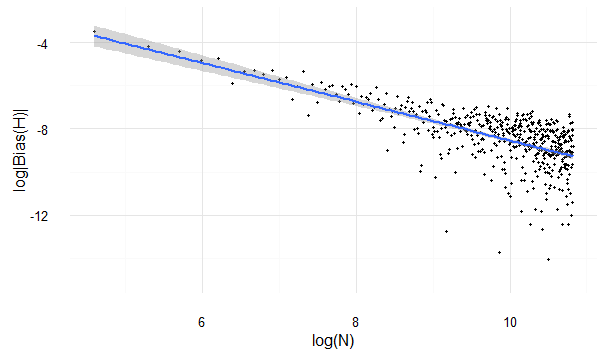
\includegraphics[width=\textwidth]{./Graphs/Best/Normal_k=6.png}\label{normal_k=6}
\caption{k=6}
\end{subfigure}%
}
\caption{1-dimensional normal distribution with different $k = 1, ..., 6$} \label{normal_graphs16}
\end{figure}


\begin{figure}
\makebox[\linewidth][c]{%
\begin{subfigure}[b]{.8\textwidth}
\centering
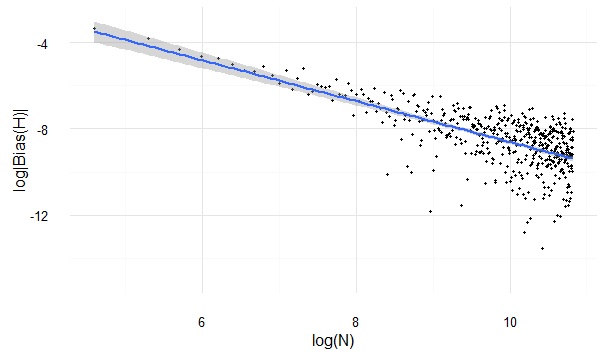
\includegraphics[width=\textwidth]{./Graphs/Best/Normal_k=7.png}\label{normal_k=7}
\caption{k=7}
\end{subfigure}%
\begin{subfigure}[b]{.8\textwidth}
\centering
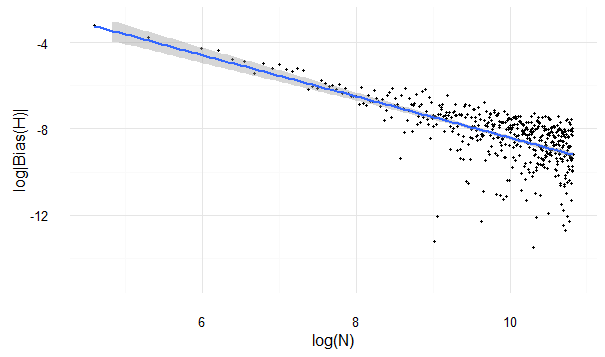
\includegraphics[width=\textwidth]{./Graphs/Best/Normal_k=8.png}\label{normal_k=8}
\caption{k=8}
\end{subfigure}%
}\    \makebox[\linewidth][c]{%
\begin{subfigure}[b]{.8\textwidth}
\centering
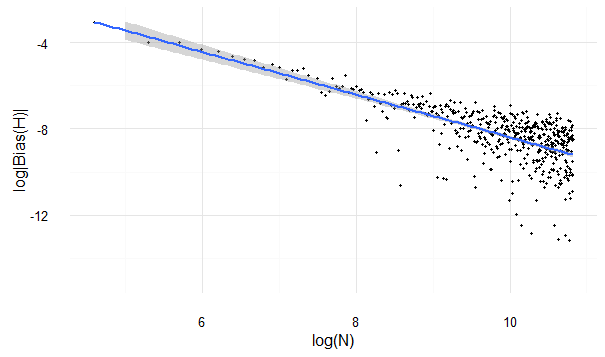
\includegraphics[width=\textwidth]{./Graphs/Best/Normal_k=9.png}\label{normal_k=9}
\caption{k=9}
\end{subfigure}%
\begin{subfigure}[b]{.8\textwidth}
\centering
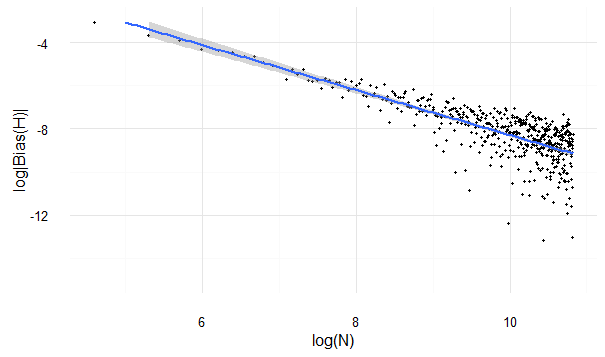
\includegraphics[width=\textwidth]{./Graphs/Best/Normal_k=10.png}\label{normal_k=10}
\caption{k=10}
\end{subfigure}%
}\    \makebox[\linewidth][c]{%
\begin{subfigure}[b]{.8\textwidth}
\centering
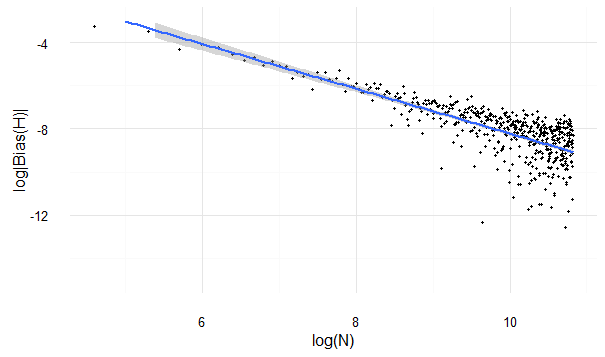
\includegraphics[width=\textwidth]{./Graphs/Best/Normal_k=11.png}\label{normal_k=11}
\caption{k=11}
\end{subfigure}%
}
\caption{1-dimensional normal distribution with different $k = 7, ...,11$} \label{normal_graphs711}
\end{figure}

Moreover, I would like to consider the coefficient of determination ($R^2$) for each of the above regression lines, this value provides an estimate of the strength of the relationship between the model and the response variable. Also, I would like to consider the standard error/deviation ($\sigma^2$), for each of the different graphs, which shows a measure of the predictions' accuracy. These are all depicted for each value of $k$ in table \ref{normal_rsq}.

\begin{table}
\caption{Comparison of the coefficient of determination and the standard deviations of the regression for each value of $k$ for the 1-dimensional normal distribution} \label{normal_rsq}
\begin{center}
\begin{tabular}{| l | c c |} 
\toprule
$k$ & $R^2$ & $\sigma^2$ \\
\midrule[1pt]
1     & 0.1766    & 1.0661    \\
2     & 0.1793    & 1.1477    \\
3     & 0.2292    & 1.1053    \\
4     & 0.3556    & 1.0759    \\
5     & 0.3322    & 1.1752   \\
6     & 0.4260    & 1.0180   \\
7     & 0.4532    & 1.0155   \\
8     & 0.4623    & 1.0088   \\
9     & 0.4962    & 0.9730   \\
10    & 0.5227    & 0.9759   \\
11    & 0.5839    & 0.8566  \\
\hline
\end{tabular}
\\[10pt]
\end{center}
\end{table}

Both columns of this table essentially point to the same conclusion; the larger the value of $k$, the more accurate the linear model is to fitting the data. This is shown by the $R^2$ value increasing towards $1$ and the $\sigma^2$ values decreasing positively. 

The $R^2$ is very small for $k \leq 3$ , which points towards the line being a poor fir to the data; however, due the the standard deviation being $\sigma^2 \approx 1.1$, we cannot say that these lines are poorly fitting; since the majority of the data is within a very small range of the line.

The most important information found from the regression analysis is shown in table \ref{normal_a_c_compare_table}; where the values of $a_{k}$ and $c_{k}$ are given for each value of $k$.

\begin{table}
\caption{Comparison of coefficients of regression $a_{k}$ and $c_{k}$ from equation \ref{bias}, for 1-dimensional normal distribution} \label{normal_a_c_compare_table}
\begin{center}
\begin{tabular}{| l | l l |} 
\toprule
$k$ &  $a_{k}$ & $c_{k}$ \\
\midrule[1pt]
1  &  0.5054 & 0.0433 \\
2  & 0.5490 & 0.0459 \\
3  & 0.6169 & 0.0894 \\
4  & 0.8181 & 0.6690 \\
5  & 0.8486 & 0.8235 \\
6  & 0.8976 & 1.5514 \\
7  & 0.9464 & 2.3576 \\
8  & 0.9574 & 3.2021 \\
9  & 0.9883 & 4.4558 \\
10 & 1.0454 & 8.5402 \\
11 & 1.0386 & 8.7457 \\
\hline
\end{tabular}
\\[10pt]
\end{center}
\end{table}

As $k$ runs from $1 \to 11$, we have that $a_{k}$ and $c_{k}$ both increase, with smooth values of $a_{k}$ and a large jump, in the value of $c_{k}$, between $k=3$ and $4$, and $k=9$ and $10$. The higher the value of $a_{k}$, the stronger the negative relationship is between the two variables in question, so for a larger values of $a_{k}$, we have that $|Bias(\hat{H}_{N, k})| \to 0$ for large $N$ faster than smaller values of $a_{k}$. This is due to the relationship between $|Bias(\hat{H}_{N, k})|$ and $a_{k}$ shown in equation (\ref{bias})

Recall, from section \ref{TODO} we have that the bias acts in one of two ways (equations \ref{fixedkbias} and \ref{dependentkbias}); it is either of $O \left( \frac{1}{N^{a}} \right)$ or $O\left( \left( \frac{k}{N} \right)^{a} \right)$. Thus we have $|Bias(\hat{H}_{N, k})|\approx \frac{c_{k}}{N^{a_{k}}}$ where either $c_{k}$ is constant or it depends on $k$ and $a_{k}$ - more specifically is $O( k^{a_{k}})$. There is evidence here to support the latter claim. If we consider the jump between $k=3$ and $4$ shown in the value of $c_{k}$, and consider the results in table \ref{normal_dependentk}. 

\begin{table}
\caption{Considering the dependence of $k$ on $c_{k}$} \label{normal_dependentk}
\begin{center}
\begin{tabular}{| l | l l l |} 
\toprule
$k$ &  $k^{a_{k}}$ & $c_{k}$ & $\frac{k^{a_{k}}}{c_{k}}$ \\
\midrule[1pt]
1  & 1 & 0.0433 & 23.095 \\
2  & 1.4631 & 0.0459 & 31.875 \\
3  & 1.9694 & 0.0894 & 22.029 \\
4  & 3.1085 & 0.6690 & 4.646 \\
5  & 3.9187 & 0.8235 & 4.759 \\
6  & 4.9942 & 1.5514 & 3.219 \\
7  & 6.3067 & 2.3576 & 2.675 \\
8  & 7.3218 & 3.2021 & 2.287 \\
9  & 8.7716 & 4.4558 & 1.969 \\
10 & 11.1020 & 8.5402 & 1.300 \\
11 & 12.0668 & 8.7457 & 1.380 \\
\hline
\end{tabular}
\\[10pt]
\end{center}
\end{table}

This shows that the proportional behaviour between $k^{a_{k}}$ and $c_{k}$ also has a large jump when $k$ goes from $3 \to 4$. This agrees with the claim of $c_{k}$ depending on $k$ in this fashion; however, in table \ref{} we mentioned another jump between $k=9$ and $k=10$, and the evidence here does not show a large jump in the same area. We cannot yet make any conclusions about the dependence of $c_{k}$ on $k$; this motivates a graphical representation of the value of $c_{k}$ against $k$ to see if there is any relation, Figure \ref{c_k_normal}.

\begin{figure}
\makebox[\linewidth][c]{%
\begin{subfigure}[b]{.8\textwidth}
\centering
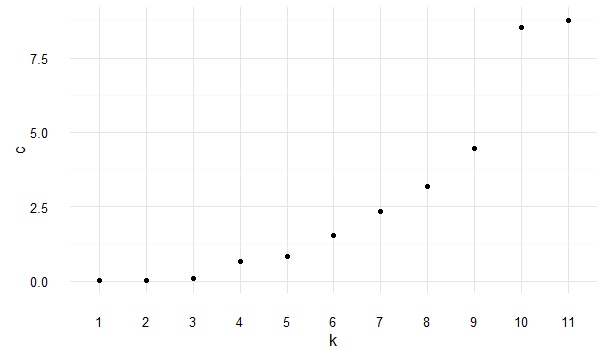
\includegraphics[width=\textwidth]{./Graphs/Best/NormalcVk.png}
\caption{The values of $k$ against the values of $c_{k}$}
\end{subfigure}%
\begin{subfigure}[b]{.8\textwidth}
\centering
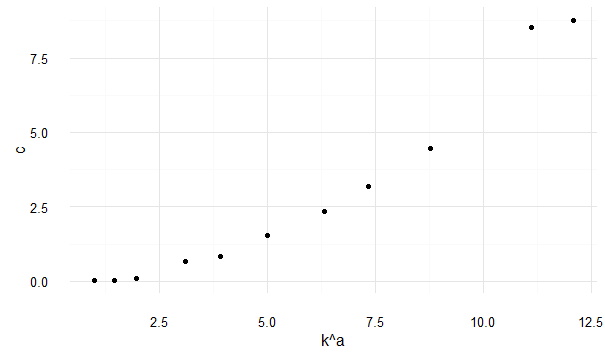
\includegraphics[width=\textwidth]{./Graphs/Best/NormalcVk2.png}
\caption{The values of $k^{a_{k}}$ against the corresponding values of $c_{k}$}
\end{subfigure}%
}
\caption{Graphically representing the relationship between $c_{k}$ and $k$} \label{c_k_normal}
\end{figure}

Interestingly, plot \ref{c_k_normal} (a) shows an almost exponential relationship between the values of $c_{k}$ and the values of $k$. This leads me to believe that there is some kind of relationship between the two variables, and looking at plot \ref{c_k_normal}(b) this shows that there's a strong possibility that the relationship is of the form stated in equation \ref{kdependentbias}.

To better study the linear relationship between the logarithm of the bias and the logarithm of the sample size, I have generated a comparison plot, shown in Figure \ref{normal_comparison_graph}. 

\begin{figure}
  \begin{center}
    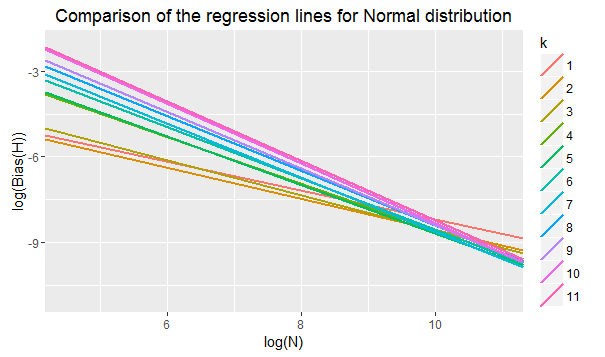
\includegraphics[width=\textwidth]{./Graphs/Best/NormalComparison.png}
  \end{center}
\caption{Plot of regression lines for $\log|Bias(\hat{H}_{N, k})|$ against $\log(N)$, for $k=1, 2,..., 11$, for samples from the normal distribution}
  \label{normal_comparison_graph}
\end{figure}

From this we can see obviously that for smaller values of $N$, smaller values of $log(N)$, the smallest bias occurs when $k=2$, since this line is the lowest for the data up until $log(N) \approx 9$ - i.e. $N \approx 13,000$. For a larger sample size, we cannot accurately see in this graph which line is the best. This motivates us to look at a section of the graph when $9 \leq log(N) \leq 11$ - i.e. $8,000 \leq N \leq 50,000$, which is shown in Figure \ref{normal_comparison_graph_zoomed}.

\begin{figure}
  \begin{center}
    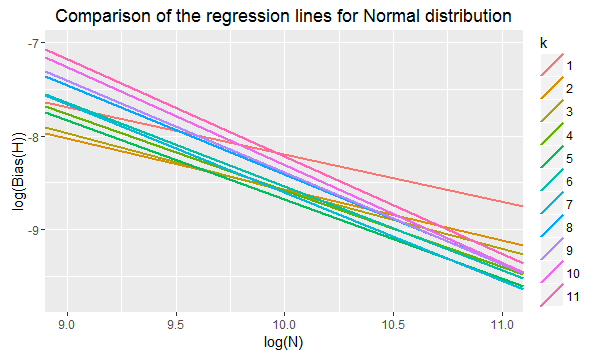
\includegraphics[width=\textwidth]{./Graphs/Best/NormalComparisonZoom.png}
  \end{center}
\caption{Figure \ref{normal_comparison_graph} zoomed in around large $N$}
  \label{normal_comparison_graph_zoomed}
\end{figure}

From this graph we can obviously discount $k=1$ for large $N$, since this is the most gradual descent; thus the bias will be largest for this $k$. Also, both the lines for $k=2$ and $k=3$ are more gradual in their descent at larger $N$, so are probably not the best to choose. Even though, for $k=9, 10$ and $11$, the slope is the steepest - $a_{k}$ is largest - the intercept is larger so around the biggest sample size considered $N=50,000$, $log(N) \approx 10.8$, there is not the smallest bias. Actually, for large values of $N \leq 50,000$ we can see from this graph that the best lines appear to be those which are blue/green; $k = 4, 5, 6, 7, 8$. Where the lowest lines around the maximal sample size are those for $k=5$ and $k=7$; thus these values of $k$ could possible be the best nearest neighbour value to choose, when looking at a sample of size $N \approx 50,000$ from the normal distribution.



















\section{1-dimensional Uniform Distribution} \label{Uniform_d=1}

I will now explore the entropy of samples from the 1-dimensional uniform distribution, $U[a, b]$. This distribution also has an exact formula to work out the entropy for. We can find this formula by considering the density function, $f$, from the uniform distribution, which is given by;
\[
f(x) =  \begin{cases} 
      \frac{1}{b-a} & a \leq x \leq b \\
      0 & otherwise
   \end{cases}
\]
Using the definition of Shannon entropy given in equation (\ref{ShaEnt}), we can find the exact entropy for the uniform distribution;
\begin{align*}
H &= - \int_{x \in \mathbb{R}^d} f(x) log(f(x)) dx \\ 
&= - \int_{a}^{b} \frac{1}{b-a} log \left[ \frac{1}{b-a} \right] dx  \\
&= - \frac{1}{b-a} log \left[ \frac{1}{b-a} \right]  \int_{a}^{b} dx  \\
&= -  log  \left[ \frac{1}{b-a} \right] 
\end{align*}
Thus, the actual value of entropy for the uniform distribution is given by;
\begin{equation} \label{UnifEnt}
H = log [ b-a ]
\end{equation}

Similarly to the 1-dimensional normal distribution, we have for the 1-dimensional uniform distribution that $d=1$ so $V_{1} = 2$, thus our estimator takes the form of equation (\ref{KLest_d=1});
\begin{equation}
\hat{H}_{N, k} =  \frac{1}{N} \sum_{i=1}^{N} log \left[ \frac{2\rho_{(k),i}(N-1)}{e^{\Psi(k)}} \right]\nonumber
\end{equation}

Moreover, the samples considered will not be from the standard uniform, but from the uniform distribution $U[0,100]$. This is because, using the standard uniform, $U[0,1]$, would fail since taking $N=50,000$ samples between 0 and 1 would generate problems as the density function would be $f(x) = 1 , \quad 0 \leq x \leq 1$, which would incur working on a very small scale; i.e taking a points with distance between them. Thus, I will be using the density function $f(x) = 0.01 , \quad 0 \leq x \leq 100$, which is from the $U[0,100]$ distribution and gives the exact entropy to be;
\begin{equation} \label{uniform_exact}
H = log(100) \approx 4.605170
\end{equation}




\subsection{Estimator Conditions} \label{U_Conditions}

For Theorems \ref{unbias} and \ref{efficient} to be satisfied by the estimators generated by samples from the uniform distribution, this density function must meet the Conditions \ref{A1}, \ref{A2} and \ref{A3}. 
Firstly, to satisfy Condition \ref{A1}, for the density function $f(x) = 0.01$ for $0 \leq x \leq 100$, it must be such that;
\begin{itemize}
\item f is bounded - obviously, since the density function for the uniform distribution is constant for $x \in [a, b]$ and $0$ otherwise; hence is bounded.

\item f is m-times differentiable - as $f$ is constant this holds

\item $\exists r_{*} > 0$ and a Borel measurable function $g_{*}$, with $\|y-x\| \leq r_{*}$ so that $\|f^{(t)}(x)\| \leq g_{*}(x) f(x)$ and $\|f^{(m)}(x) - f^{(m)}(x)\| \leq g_{*}(x) f(x)\|y - x\|^{\eta}$, for some $g_{*}$ such that $\sup_{\{x : f(x) < \delta\}} g_{*}(x) = O(\delta^{-\epsilon})$ as $\delta \searrow 0$ for some $\epsilon >0$.
Since we are considering a 1-dimensional distribution, we can write the norms $\| \cdotp \|$ as  $| \cdotp |$. Moreover, considering that for Theorems \ref{unbias} and \ref{efficient}, we have the value of $\beta \geq 2$; thus choosing $\beta = 2$, and since $m = \lfloor \beta \rfloor =  \lfloor 2 \rfloor = 2 = \beta$ and $\eta = \beta -m$, we have that $\eta =0$. Thus we need  $|f^{(t)}(x)| \leq g_{*}(x) f(x)$, which is obvious since $f$ is constant for $f^{(t)}(x) = 0$ for all $t \geq 1$ TODO - sort this out

\end{itemize}

Next, to satisfy Condition \ref{A2}, for the density function $f$ of the uniform distribution, must fulfill that;
\begin{itemize}
\item The $\alpha$-moment of $f$ must be finite, so $\int_{\mathbb{R}^{d}} \| x \|^{\alpha} f(x) dx < \infty$ - this is true, since for the 1-dimensional uniform distribution, $f(x)$ is constant; thus we would be integrating a polynomial $|x|^{\alpha}$, over a finite interval $a \leq x \leq b$, which is always finite.
\end{itemize}

Lastly, to satisfy Condition \ref{A3}, we must find the values of $k$ for which the estimator provides a uniform convergence for Theorems \ref{unbias} and \ref{efficient}. These values are independent of the distribution that the sample is from, and only depends on the size of the sample, the dimension of the distribution that sample is taken from and the value chosen for $\alpha$, where we have chosen $\alpha = 2$. The values of $k$ found in section \ref{N_Conditions} are $\{1,2\}$ for $N=100$, $\{1, 2, ..., 9\}$ for $N=25,000$ and then $\{1, 2, ..., 11\}$ for $N=50,000$. 

Thus, due to the above conditions for Theorems \ref{unbias} and \ref{efficient} being met, we can say that the Kozachenko-Leonenko estimator, of a sample from the uniform distribution is an asymptotically unbiased and consistent estimator for entropy, for specific $k \in \{1, 2, ..., 11 \}$, depending on the sample size $N$.




\subsection{Simulation Results}

I will now conduct simulations, in a similar manner as for the normal distribution, where for each value of $k$ separately, I will consider $500$ samples of size $N$ from the uniform distribution, finding the estimator in each case and take the average of these estimators to find our entropy estimator. I will then consider the relationship show in equation (\ref{logbias}) for each sample and work out the average for the values of a and c, for each $k \in \{1, 2, ..., 11\}$. 

For $N=100$, $N=25,000$ and $N=50,000$, using the results from \ref{TODO-appendix data}, we can create a table to compare the mean values of the bias of the estimator for the different values of $k$ considered. 

\begin{table}
\caption{1-dimensional uniform distribution, comparison of $k$} \label{uniform_kcompare_table}
\begin{center}
\begin{tabular}{| l | c c c |} 
\toprule
$k$ &  $|Bias(\hat{H}_{100, k})|$ & $|Bias(\hat{H}_{25000, k})|$  &  $|Bias(\hat{H}_{50000, k})|$ \\
\midrule[1pt]
1     & 0.0005189    &       Inf    &       Inf   \\
2     & 0.0047466    & 0.0001745    & 0.0001163   \\
3     & 0.0083912    & 0.0001776    & 0.0000899   \\
4     & 0.0169364    & 0.0001177    & 0.0000490   \\
5     & 0.0152168    & 0.0000588    & 0.0000509   \\
6     & 0.0148205    & 0.0000817    & 0.0000538   \\
7     & 0.0218339    & 0.0002918    & 0.0000663   \\
8     & 0.0250401    & 0.0001884    & 0.0000487   \\
9     & 0.0297655    & 0.0001406    & 0.0001184   \\
10    & 0.0337164    & 0.0001337    & 0.0000949   \\
11    & 0.0381473    & 0.0001693    & 0.0000417   \\
\hline
\end{tabular}
\\[10pt]
\caption*{This table is comparing the values of $|Bias(\hat{H}_{N, k})|$ for the values of $k$ with $N=100$, $N=25,000$ and $N=50,000$, when the estimator is taken over $500$ samples}
\end{center}
\end{table}

Looking at the results shown in table \ref{uniform_kcompare_table}, for $N=100$, we can see that the smallest bias, quite obviously, occurs when the estimator is taken with $k=1$, and that for other values of $k$ there is a significant difference in the size of the bias.

When looking at the larger values of $N$, it is first important to note that \texttt{Inf} $= \infty$ is present in the table as for a large value of $N$, it is difficult to work out the estimator when $k=1$. This is because there are only extremely small distances between the closest samples of this distribution, and since any program used to compute these numbers will fail with extremely small numbers and default them to \texttt{- Inf}. We only need there to be two samples with an infinitely small distance to make the whole estimator become \texttt{- Inf}, which is \texttt{Inf} when looking at the modulus. This was mentioned earlier and was the motivation for taking the uniform distribution over $[0, 100]$; however, because of this, from now onwards I will not be considering $k=1$ in the estimator for the uniform distribution.

Thus, looking at the results shown in table \ref{uniform_kcompare_table}, ignoring $k=1$ and considering $N=25,000$, it appears to show smallest bias for values of $k \in \{4, 5, 6 \}$; more specifically $k=5$ appears to have the smallest bias. This fits with the previous analysis done on the value of $k$ for different sample sizes, which stated that we must have $k \in \{1, 2, ..., 9\}$. Next, examining the table for $N=50,000$, we can see that the smallest bias looks to be when $k \in \{ 4, 5, 6, 7, 8, 11\}$, however, for all other values of $k$ we still have a small bias $< 0.000012$. Thus, we cannot yet draw any conclusions about the optimal value of $k$ for large $N$ and this distribution.

Next I wish to examine the graphs showing the relationship in equation \ref{logbias}, by plotting the simulated data and fitting a regression line for each value of $k$ separately, in figures \ref{Uniform_graphs27} and \ref{Uniform_graphs811}. Thus showing a negative linear relationship between the logarithm of the bias of the estimator and the logarithm of the sample size $N$. Also, looking more closely, the regression lines fitted to the data appear to become more steep for higher values of $k$, whilst the standard error bars appear to become smaller. 

\begin{figure}
\makebox[\linewidth][c]{%
\begin{subfigure}[b]{.8\textwidth}
\centering
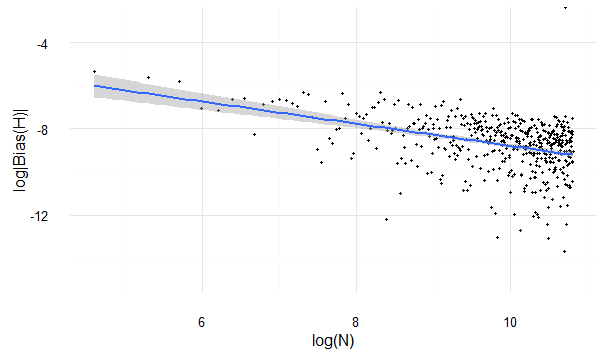
\includegraphics[width=\textwidth]{./Graphs/Best/Uniform_k=2.png}
\caption{k=2}
\end{subfigure}%
\begin{subfigure}[b]{.8\textwidth}
\centering
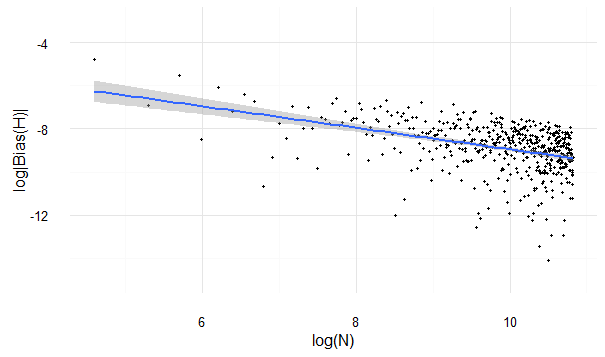
\includegraphics[width=\textwidth]{./Graphs/Best/Uniform_k=3.png}
\caption{k=3}
\end{subfigure}%
}\    \makebox[\linewidth][c]{%
\begin{subfigure}[b]{.8\textwidth}
\centering
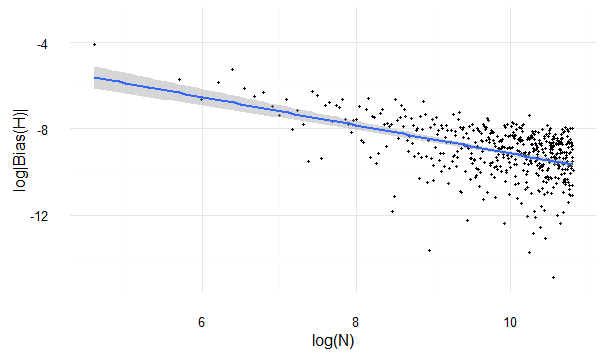
\includegraphics[width=\textwidth]{./Graphs/Best/Uniform_k=4.png}
\caption{k=4}
\end{subfigure}%
\begin{subfigure}[b]{.8\textwidth}
\centering
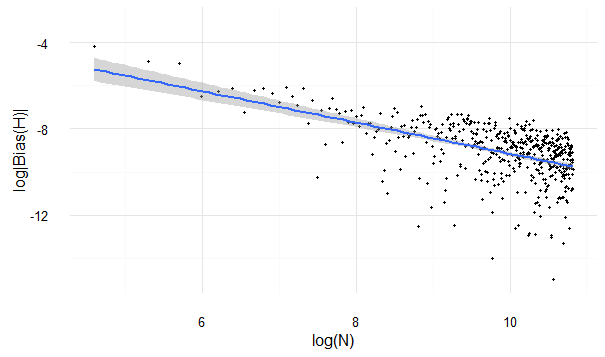
\includegraphics[width=\textwidth]{./Graphs/Best/Uniform_k=5.png}
\caption{k=5}
\end{subfigure}%
}\    \makebox[\linewidth][c]{%
\begin{subfigure}[b]{.8\textwidth}
\centering
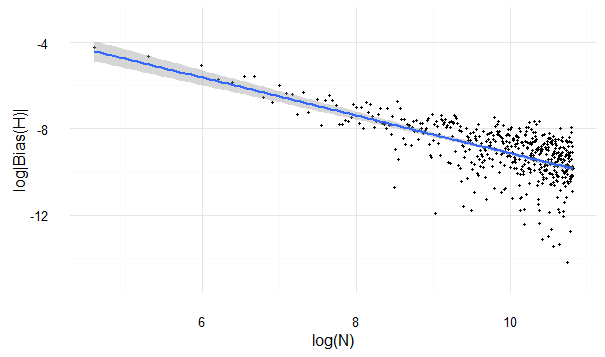
\includegraphics[width=\textwidth]{./Graphs/Best/Uniform_k=6.png}
\caption{k=6}
\end{subfigure}%
\begin{subfigure}[b]{.8\textwidth}
\centering
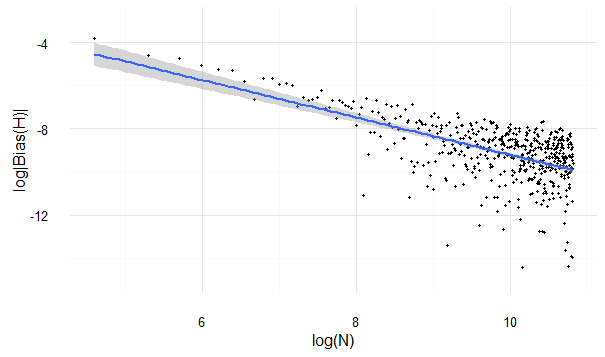
\includegraphics[width=\textwidth]{./Graphs/Best/Uniform_k=7.png}
\caption{k=7}
\end{subfigure}%
}
\caption{1-dimensional Uniform distribution with different $k = 2, ..., 7$} \label{Uniform_graphs27}
\end{figure}


\begin{figure}
\makebox[\linewidth][c]{%
\begin{subfigure}[b]{.8\textwidth}
\centering
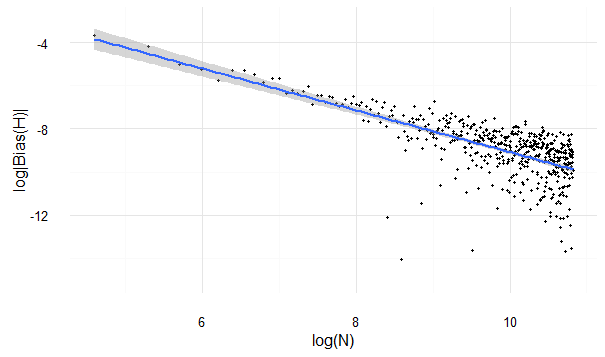
\includegraphics[width=\textwidth]{./Graphs/Best/Uniform_k=8.png}
\caption{k=8}
\end{subfigure}%
\begin{subfigure}[b]{.8\textwidth}
\centering
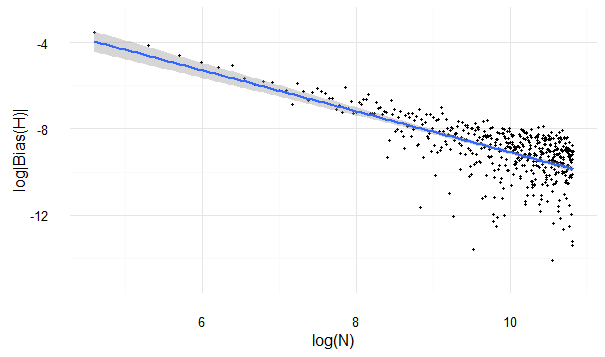
\includegraphics[width=\textwidth]{./Graphs/Best/Uniform_k=9.png}
\caption{k=9}
\end{subfigure}%
}\    \makebox[\linewidth][c]{%
\begin{subfigure}[b]{.8\textwidth}
\centering
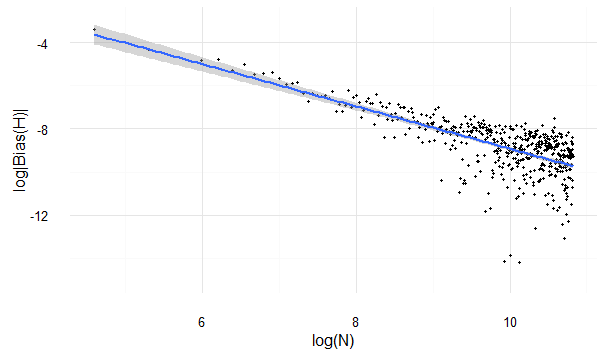
\includegraphics[width=\textwidth]{./Graphs/Best/Uniform_k=10.png}
\caption{k=10}
\end{subfigure}%
\begin{subfigure}[b]{.8\textwidth}
\centering
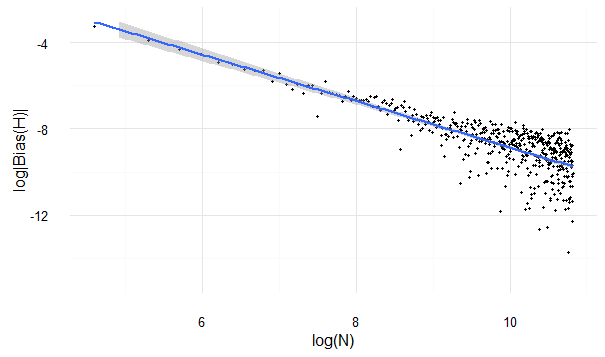
\includegraphics[width=\textwidth]{./Graphs/Best/Uniform_k=11.png}
\caption{k=11}
\end{subfigure}%
}
\caption{1-dimensional Uniform distribution with different $k = 8, ...,11$} \label{Uniform_graphs811}
\end{figure}

Another important thing to consider, before looking at the equations of the regression lines, is to see how well these lines actually fit the data. To do this I have, as before, examined the coefficient of determination and the standard deviation of the lines, Table \ref{uniform_rsq}.

\begin{table}
\caption{Comparison of the coefficient of determination and the standard deviations of the regression for each value of $k$ for the 1-dimensional uniform distribution} \label{uniform_rsq}
\begin{center}
\begin{tabular}{| l | c c |} 
\toprule
$k$ & $R^2$ & $\sigma^2$ \\
\midrule[1pt]
2     & 0.1721    & 1.0982   \\
3     & 0.1576    & 1.1402   \\
4     & 0.2485    & 1.1200   \\
5     & 0.2784    & 1.1459   \\
6     & 0.4027    & 1.0286   \\
7     & 0.3605    & 1.1252   \\
8     & 0.4689    & 1.0073   \\
9     & 0.4653    & 0.9940   \\
10    & 0.5088    & 0.9408   \\
11    & 0.6215    & 0.8208   \\
\hline
\end{tabular}
\\[10pt]
\end{center}
\end{table}

This table is very similar to that for the normal distribution in that both columns point towards the same conclusion; the larger that $k$ is, the more accurate the linear model is to fitting the data. This is shown by the $R^2$ value generally increasing towards $1$ and the $\sigma^2$ values decreasing positively - the deviation about the line is decreasing for higher $k$. There is slight fluctuation in the middle values of $k$, where for $k = \{6, 7, 8\}$ there is not an exact direction that the relationship is going. However, there is nothing to say that this isn't normal behaviour, since we do not yet know the relationship between the bias and $k$.

Moreover, $R^2$ is very small for $k \leq 4$ , which points towards the line being a poor fir to the data; however, due the the standard deviation being $\sigma^2 \approx 1.1$, we cannot discard the importance of these lines; since most of the data is in a very small range about the line. Additionally, for $k=11$ we have the strongest relationship seen so far - the largest $R^2$ and smallest $\sigma^2$ values appear - this could indicate that for this distribution, when $k=11$ the linear relationship between the logarithm of the bias and the logarithm of the sample size is most likely to be true.

Possibly the most important information found from the regression analysis, is shown in Table \ref{uniform_a_c_compare_table}; where the values of $a_{k}$ and $c_{k}$ are given for each value of $k = \{ 2, 3, ..., 11\}$.

\begin{table}
\caption{Comparison of coefficients of regression $a_{k}$ and $c_{k}$ from equation \ref{bias}, for 1-dimensional uniform distribution} \label{uniform_a_c_compare_table}
\begin{center}
\begin{tabular}{| l | l l |} 
\toprule
$k$ &  $a_{k}$ & $c_{k}$ \\
\midrule[1pt]
2     & 0.5125    & 0.0258   \\
3     & 0.5048    & 0.0199   \\
4     & 0.6593    & 0.0779   \\
5     & 0.7286    & 0.1531   \\
6     & 0.8645    & 0.6090   \\
7     & 0.8648    & 0.5758   \\
8     & 0.9688    & 1.8377   \\
9     & 0.9492    & 1.5095   \\
10    & 0.9801    & 2.4041   \\
11    & 1.0765    & 6.6932   \\
\hline
\end{tabular}
\\[10pt]
\end{center}
\end{table}

We wish to have a value of $a_{k} \geq 0.5$ to show the relationship desired, and this is true for all values of $k$ in this table. As $k$ increases, we have that both $a_{k}$ and $c_{k}$ increase, expect for $k=8$, which has larger values that $k=9$. However, this slight change around $k=8$ does not necessarily imply anything dramatic since the overall trend seems to fit with that found for the normal distribution.

TODO - talk about $a_{k}$ and $c_{k}$ in table \ref{uniform_a_c_compare_table}

TODO - talk about graph in Figure \ref{uniform_comparison_graph}


\begin{figure}
  \begin{center}
    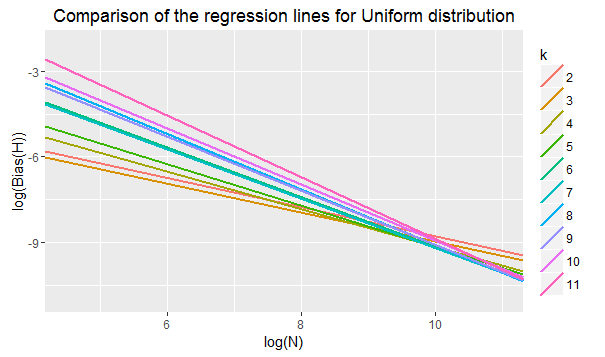
\includegraphics[width=\textwidth]{./Graphs/Best/UniformComparison.png}
  \end{center}
\caption{Plot of regression lines for $\log|Bias(\hat{H}_{N, k})|$ against $\log(N)$, for $k=2, 3,..., 11$, for samples from the uniform distribution}
  \label{uniform_comparison_graph}
\end{figure}


\end{document}